\documentclass[tikz,border=10pt]{standalone}
% Scale s = 0.014953 cm/px (STYLE METRICS), origin at ink-bbox centre (305,243)
\usepackage{tikz}
\begin{document}
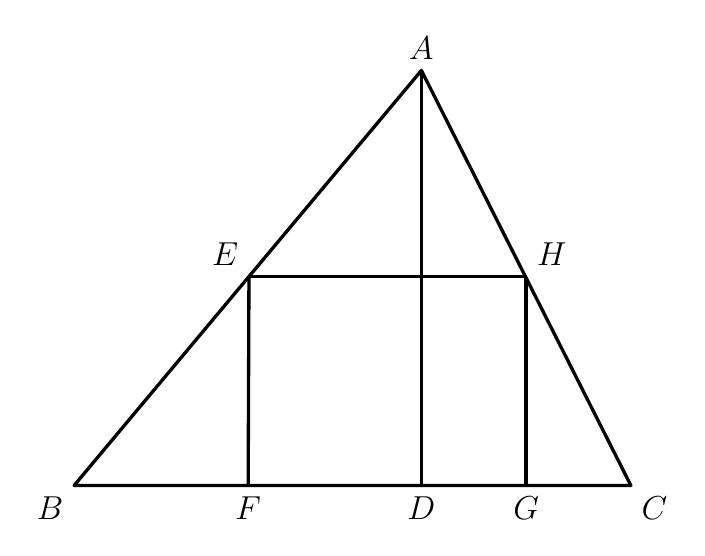
\begin{tikzpicture}[line join=round, line width=1.2pt, every node/.style={font=\fontsize{12}{14.4}\selectfont}]

% Vertices (TikZ cm)
\coordinate (A) at (0.88,2.62);
\coordinate (B) at (-3.53,-2.65);
\coordinate (C) at (3.54,-2.65);
\coordinate (D) at (0.88,-2.65);
\coordinate (F) at (-1.32,-2.65);
\coordinate (G) at (2.21,-2.65);
\coordinate (E) at (-1.31,0);
\coordinate (H) at (2.21,0);

% Triangle ABC
\draw (A) -- (B) -- (C) -- cycle;

% Interior segments (stop at vertices)
\draw (E) -- (H);   % horizontal E-H
\draw (E) -- (F);   % vertical E-F
\draw (H) -- (G);   % vertical H-G
\draw (A) -- (D);   % altitude A-D

% Labels
\node[above] at (A) {$A$};
\node[below left] at (B) {$B$};
\node[below right] at (C) {$C$};
\node[below] at (D) {$D$};
\node[below] at (F) {$F$};
\node[below] at (G) {$G$};
\node[above left] at (E) {$E$};
\node[above right] at (H) {$H$};

\end{tikzpicture}
\end{document}